\section{Result}
\label{sec:result}
Inside this section the principle results of my work are illustrated. Note that
the absolute performance values depends strongly on the hardware of the machine used.
All the tests were run on a Intel(R) Core(TM) i7-3610QM CPU @ 2.30GHz.

In order to show the performance and the differences between the two implementations I selected some files
that can be found in the \verb|/Sample| directory.

Each instance was run ten times and the average
user time was computed.
This measure was preferred over the cpu time,
for two reasons:
\begin{itemize}
	\item because the CPLEX solution is multi-threaded it requires
	circa 6-7 times more cpu time than the one-thread genetic algorithm.
	\item a company that produces drill boards is more interested in the wall clock time than the cpu one.
\end{itemize} 

\subsection{Benchmark description}
The instances used during the test are the following:
\begin{itemize}
	\item TSP12, the tsp instance with 12 elements given during the class;
	\item TSP60, the tsp instance with 60 elements given during the class;
	\item REALWORLD, the real-world tsp instance, with data extrapolated from a real-world
	\verb|.gbr| file mentioned above in section \ref{sec:Gerber}.
	\item CIRCLE3-50 Circle instances 3 to 50 (See chapter \ref{sec:instance:generator})
	\item RANDOM3-50 50 random but fixed instances, used in order to show the general-purpose efficiency of the genetic algorithms and the quality of the provided solutions;
	\item RANDOM100a and RANDOM100b, two random but fixed instances
	in order to show the general-purpose efficiency of the genetic algorithm and observe that the exact solution is well-suited
	for (even reasonably big) random instances.
\end{itemize}
During the rest of the paper the names of the tests will be fixed.
\newpage
\section{Result - First Assignment}
In this part of the report the focus is mainly  on the performance of the exact solution. 
In general the variance between the different exact solution runs
is negligible and therefore these data are not reported.

Now follow the considerations about the single benchmarks:

\paragraph{CIRCLE3-50}
The results provided by this benchmark can be seen in figure \ref{subfig:circle_performance}. They are quite surprising because
the time does not grow (always) proportionally with the increase of $N$.
Note especially the entries 37,41,47 require a very small amount of time. Instead
there are also inputs with which CPLEX cannot deal easily, such as 46, that was not reported in the graph because it required 23 minutes,
49 that is not reported because after circa 1 hour it did not return back a result.

\paragraph{RANDOM3-50}
The result of this benchmark (figure \ref{subfig:random_performance}) shows that, when $N$ increases, the required time 
grows accordingly, especially from $36$ on.
Even though there are some exceptions, because of the
lack of a strong relationship between the random instances, the trend is evident.

\paragraph{TSP12, TSP60, RealWorld}
The TSP60 and the RealWorld examples consist of circa the same number of points and
therefore the required  time lies in the same order of magnitude as shown in figure
\ref{fig:sub:tsp60RealWorld}.

\paragraph{Random100a, Random100b}
The results can be viewed on figure \ref{fig:sub:tsprandom100ab}. They show that 
the exact algorithm works well particularly with random instances.

\begin{figure}[h]
	\centering
	\begin{subfigure}{.4\textwidth}
	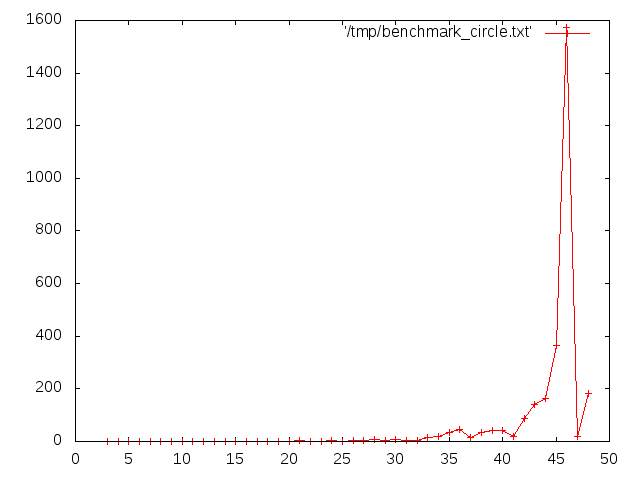
\includegraphics[width=1\linewidth]{img/benchmark_circle.png}
	\caption{}
	\label{subfig:circle_performance}
	\end{subfigure}
	\begin{subfigure}{.4\textwidth}
	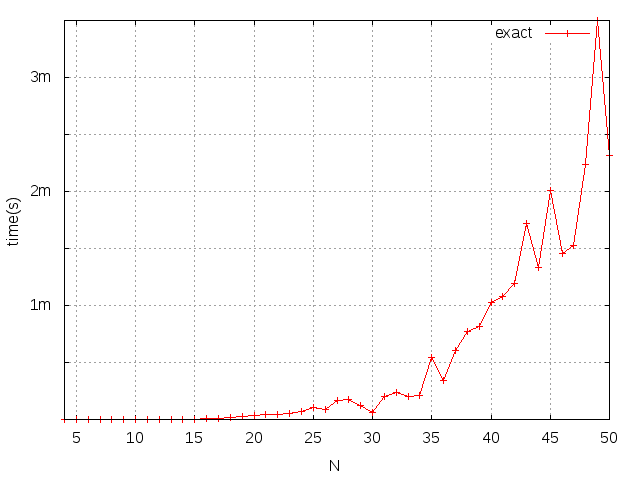
\includegraphics[width=1\linewidth]{img/firstAssignment/RANDOMTSPINSTANCE.png}
	\caption{}
	\label{subfig:random_performance}
	\end{subfigure}
	\caption{The time result of the benchmark CIRCLE3-50, RANDOM3-50}
\end{figure}



\begin{figure}
		\centering
		\begin{subfigure}{.45\textwidth}
				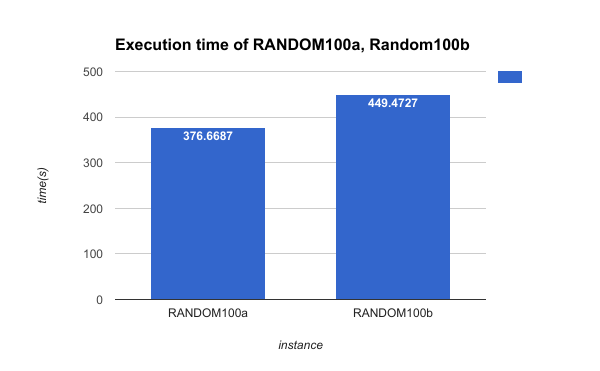
\includegraphics[width=1\linewidth]{img/TSPRANDOM100a-bTIme.png}
			\caption{}
						\label{fig:sub:tsprandom100ab}
		\end{subfigure}
		\begin{subfigure}{.45\textwidth}
			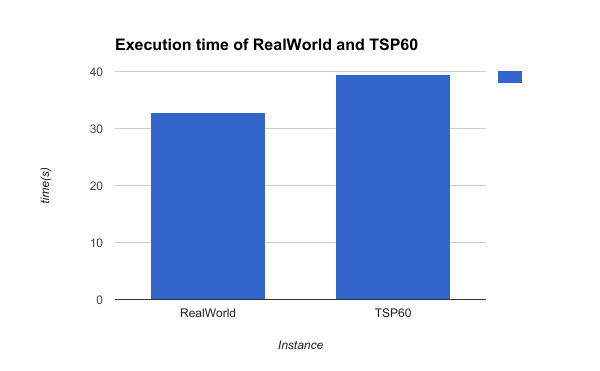
\includegraphics[width=\linewidth]{img/firstAssignment/TSP60RealWorld.png}		
			\caption{}
						\label{fig:sub:tsp60RealWorld}

		\end{subfigure}
		
		\caption{The time result of the benchmark Random100a and Random100b}
		
\end{figure}

\paragraph{Considerations.}
In general from the above graphs I concluded:
\begin{itemize}
	\item That with a small $N$ (from 3 to 30) the program performs blazingly fast.
	\item The program works better with solutions that are generated randomly, i.e. with points distributed 
	across the whole board. Instead it requires (generally) more time when the points are grouped
	in the corners of the board. In this case 
	we can observe that the performance of the exact algorithm becomes very unstable, you can consider $N = 46$ and $N=47$ as an example
	(See figure \ref{subfig:circle_performance}).
	
\end{itemize}
\newpage


\section{Result-Second Assignment}
\label{sec:II:performance}
This section is divided into two
parts: the first analyzes the time required by the algorithm 
and the stability of the results provided with different configurations for
$S$, the population size.


This algorithm relies on the random choices made during the execution and on other factors such as the population size.

\paragraph{Note about the tuning of the algorithm} Note that $R$, the number of new individuals generated in each iteration, is dependent on $S$. It is obtained
as the ceiling of the square root of $S$\footnote{If this number is odd it is incremented.}. This implies that $R << S$ and therefore the selection sort works excellently.

In order to choose the population size I tested TSPRANDOM100a-b, TSP12, REALWORLD and TSP60 10 times with population $10$ and population $100$.
The main results are summarized in the tables \ref{table:valuestability} and \ref{table:timestability}.
As you can see in the last line of table \ref{table:valuestability} the standard deviation of the values, is very low.
Since the calculated average value are substantially equivalent the population size $10$ was preferred
for its efficiency, that is 7-8 times faster than the other configuration. 
\begin{table}
	\begin{tabular}{| l || l | l || l | l| l | }
		\hline
		Instance 		& Time CV - 10 & AVG - 10  & Time CV - 100 & AVG - 100 & ratio  \\
		\hline
		TSP12    		& 31.78\%           &    0.04     & 24.62\% &  0.40 & 10\\
		TSP60    		& 13.77\%           &  	 0.52	  & 28.77\% &  4.55 & 8.75\\
		REALWORLD		& 9.50\%            &  	 0.30	  & 28.25\% &  1.83 & 6.1\\
		TSPR100a 		& 20.70\%	        	&  	 1.25	  & 24.72\% &  10.64 & 8.51\\
		TSPR100b 		& 20.33\%				&  	 1.23	  & 18.84\% &  11.56 & 9.39\\
		\hline
		Average			&		19.2\%		&			  &	25.04\%	&		 & 8.55\\
		\hline
	\end{tabular}
	\caption{Comparison about the time performance, when using 10 or 100 as population size.}
	\label{table:timestability}
\end{table}

\begin{table}
	\begin{tabular}{| l || l | l || l | l| l |}
		\hline
		Instance 		& Value CV - 10 & AVG - 10  & Value CV - 100 & AVG  - 100 & ratio \\
		\hline
		TSP12    		& 0.0\%             &    66.4     & 0.0\% 	&  66.4 & 1.0 \\
		TSP60    		& 6.64\%            &  	 836.54	  & 5.04\% 	& 832.99 & 0.995\\
		REALWORLD		& 4.34\%            &  2.94E+08	    & 4.93\% &  2.83E+08 & 0.963\\
		TSPR100a 	& 6.37\%	        &  	 16,726.31  & 7.39\% &  16,872.59 & 1.008\\
		TSPR100b 	& 8.75\%			&  	 16,320.84	  & 9.67\% &  16,728.37 & 1.024\\
		\hline
		Average    &    5.22\%          &                   & 5.40\%  &            & 0.99 \\
		\hline 
	\end{tabular}
	\caption{Comparison about the stability of the algorithm, i.d. in the variance of the values and average values.}
	\label{table:valuestability}
\end{table}
 


\newpage
\section{Comparison between Solution I and Solution II}
It does not make too much sense to compare the metaheuristic and the
exact approach on a time based, because the genetic algorithm is tremendously faster
as described in figure \ref{fig:comparison}.


\begin{figure}
	\centering
	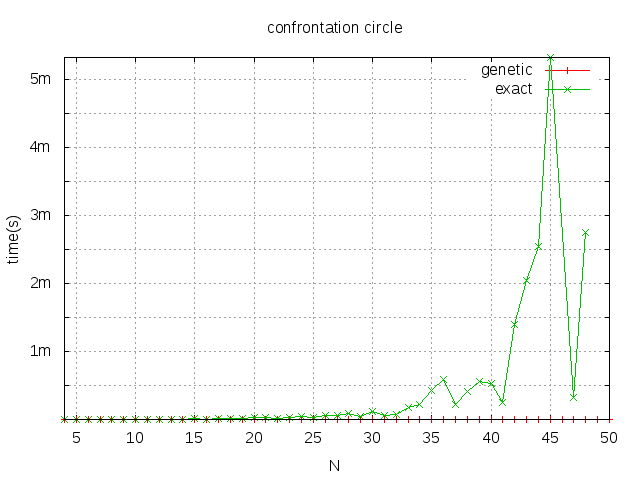
\includegraphics[scale=0.42]{img/confronto_circle_exact_genetic.png}
	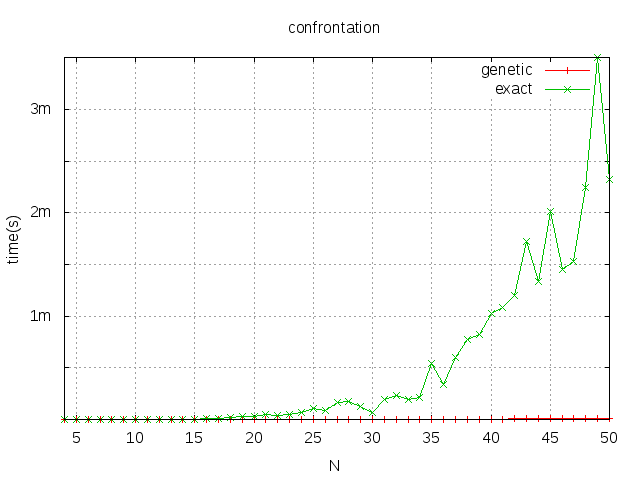
\includegraphics[scale=0.42]{img/confronto_random_exact_genetic.png}
	\caption{Comparison between exact and genetic algorithm on a time basis.}
	\label{fig:comparison}
\end{figure}



\subsection{Quality of the result}
Inside this section the result provided by the genetic algorithm are compared with
those generated by the exact solution.
In the table \ref{table:quality}  the results given by the genetic algorithm are compared
with the optimal solutions.
As seen in the previous section the algorithm is quite stable and with small instances
it can provide very good solutions compared to the optimal solutions, as summarized in the table
\ref{table:quality} with an error of circa 20 \%.
it can find
good values compared to the optimal solutions, as summarized in the table \ref{table:quality}.
But with the increasing of $N$ the precision becomes worse and worse.
\begin{table}
	\centering
\begin{tabular}{|l|r|r|r|r|}
	\hline
	Instance 	& Exact Solution & AVG Error &  Worst Case & Best Case  \\
	\hline
	TSP12 		&  	66.4		   &  0\%	   		&	0\%	     	&     0\%   \\
	TSP60 		&  	629.8		   &  	32.83\%     &	42.60\%		&    17.99\% \\
	REALWORLD 	&   222811276      & 	31.89\%   	&	37.65\%   	&   24.32\% 	    \\
	TSPRANDOM100a & 9778.91        & 71.04\% 		& 	87.75\% 	& 51.17 \% \\
	TSPRANDOM100b & 9802.71        & 66.50\% 		&	83.28\% 	& 42.50\% \\
	\hline
\end{tabular}
\caption{In this table the result of the comparison are formalized. The coefficient of variation is used to show
	the deviation between the $10$ computed result.}
\label{table:quality}
\end{table}
